\documentclass[11pt]{article}
\usepackage{geometry}                
\geometry{letterpaper}                   

\usepackage{graphicx}
\usepackage{amssymb}
\usepackage{epstopdf}
\usepackage{natbib}
\usepackage{amssymb, amsmath}
\DeclareGraphicsRule{.tif}{png}{.png}{`convert #1 `dirname #1`/`basename #1 .tif`.png}
\usepackage{listings}
\usepackage[latin1]{inputenc}   
\usepackage{pdfpages}
\usepackage{url}
\usepackage{subfloat}

\urlstyle{same}

\newcommand{\dis}{\displaystyle}
\newcommand{\noi}{\noindent}
\newcommand{\y}[1]{\text{#1}}
\newcommand{\erw}[1]{\langle #1 \rangle}
\newcommand{\brac}[1]{\dis \left(#1\right)}

\title{Pedestrian dynamics in long, narrow hallways}
\author{Moser Manuel, Suter Yannick, Theiler Raffael}
\date{December 2012} 

\begin{document}

%COVER
\thispagestyle{empty}

\begin{center}

\includegraphics[width=5cm]{ETHlogo.eps}

\bigskip
\bigskip
\bigskip


\LARGE{ 	Lecture with Computer Exercises:\\ }
\LARGE{ Modelling and Simulating Social Systems with MATLAB\\}

\bigskip
\bigskip

\small{Project Report}\\

\bigskip
\bigskip
\bigskip
\bigskip


\begin{tabular}{|c|}
\hline
\\
\textbf{\LARGE{Pedestrian dynamics in long, narrow hallways}}\\
%\textbf{\LARGE{...}}\\
\\
\hline
\end{tabular}

\bigskip
\bigskip
\bigskip

\LARGE{Moser Manuel, Suter Yannick \& Theiler Raphael}
\vfill
Zurich\\
December 2012\\

\end{center}
\newpage

%Agreement for free download
%Agreement for free download
%not (yet) changed in any way, simply copied it out from the main file.

\section*{Agreement for free-download}
\bigskip


\bigskip


\large We hereby agree to make our source code for this project freely available for download from the web pages of the SOMS chair. Furthermore, we assure that all source code is written by ourselves and is not violating any copyright restrictions.


\begin{center}
\vspace{3cm}
Moser Manuel \hspace{3cm} Suter Yannick \hspace{3cm} Theiler Raffael

\end{center}


\newpage

%ETH declaration of originality
%Link: http://www.ethz.ch/faculty/exams/plagiarism/index_EN

\begin{figure}
	\centering
	
\includegraphics[width=0.9\textwidth]{declaration_print.pdf}
	\label{fig:declaration}
\end{figure}
\clearpage


%Table of Contents
\tableofcontents
\newpage

%All those in seperate Files just need to be imported back in again.

\section{Abstract}
%Abstract

Authors: Manuel Moser, Yannick Suter, Raffael Theiler\\
Title: Pedestrian dynamics in long, narrow hallways\\
\\
In this project, we want to have a closer look at pedestrians in narrow hallways, motivated by a situation at Zurich main station. To do this, we simulate pedestrians by agents with Matlab who walk according to some rules. We managed our agents to pass each other by, to look ahead a few meters and to decide where to walk next.\\
At first, we wanted to have a closer look at the pedestrian flux when the number of persons per minute entering is increased, when there are clearly more people moving in the same direction against a few in the other direction. Next, we wanted to analyze the influence of aggressive fast people in a rush, slowly moving obstacles and the influence of drunkard (randomized walking) on the pedestrian flux.\\
But soon, our attention turned more to building/creating everything on our own and less about a fast simulation of different situations.\\
The main outcome of our simulations was that pedestrians tend to get stuck or create jams as soon as there are lots of people trying to pass the same hallway. The exact same hallway can work smoothly if there are not too many people, but jams can arise quickly. And once a jam starts, it often spreads out because people have to stop and walk slower.\\
Finally, we arrived at the following conclusions: To improve the pedestrian flux, broadening a hallway is a superb solution. Therefore, at our situation scene at Zurich main station, it would be best if the hall users would try to leave more space for the pedestrians, and if the food shops Imagine and Nordsee wouldn't have chairs and tables outside.

\newpage

\section{Individual contributions}
%IndividualContributions

\begin{tabbing}
Contributor \= \kill
Manuel: \> coordination, report, revising \& graphics/plots \\
Yannick: \> logical functions, revising, debugging \& matlab overview \\
Raffael: \> graphical functions, visualization \& agents \\
\end{tabbing}

\noi Listed above are only the main tasks everyone of us took care of, but we shared most of the work. The github commit report is not always mirroring the work behind those uploads because we often worked together on the code, debugged, commented and worked on the documentation while swapping laptops.

\newpage

\section{Introduction and Motivation}
%IntroductionAndMotivation

%evtl. irgendwo Anmerkung machen dass ich hier mich ziemlich an den Research Plan halte (motivation, fundamental questions anfang & expected results sehr �hnlich)?

%Add Oktoberfest-Situation-Picture and main station situation sketch in this section (the main station sketch also in the model/implementation section)

\subsection{Motivation}
As many commuters too, we all got annoyed by people rushing through the small corridor left in Zurich main station hall (the path between burger king and groups meeting point) during the Oktoberfest, market days, concerts and other occasions. So when thinking about a simulation project, this quickly crossed our minds. Special about this situation of a narrow but long corridor is that there's not much space to avoid other pedestrians to the side, especially if there are lots of other people whereas there is no need of path optimisation as the ultimate goal is to cross the hallway without crashing into someone else.
%Add Oktoberfest-Situation-Picture here

\subsection{Fundamental Questions}
The fundamental questions of our simulation project we started with are:
\begin{itemize}
\item We try to simulate the pedestrian flux of agents in a hallway in the following different situations: Rush hour (danger of jamming), much more agents in one direction than in the other, with an static obstacle (if possible), with aggressive/very fast or slow agents, random path agent (drunkard). Will the pedestrian flux run smoothly or will they block each other and be stuck?
\item Will the implementation of a rudimentary kind of thinking/looking ahead help to avoid blockages? If possible, we may determine the limits for which the goal of passing is achieved with and without this implementation and compare them.
\item Will there be group dynamics or similar behaviours of agents even if they're only programmed to walk to the other side, each on his own?
\end{itemize}

As soon as the programming phase started, we realized there was a major point of importance about this work we all were aware of, but had forgot to think about beforehand. We did not want to start with a simulation already created, but build something "new". So we started off creating our logic function that would allow the agents to avoid crashing into other agents. So, new fundamental questions arised:
\begin{itemize}
\item Starting with the idea of looking ahead, how can we turn this into a rudimentary kind of intelligence?
\item How can we have a look at the main station situation but keep our agents as random as possible?
\end{itemize}

\subsection{Expected Results}
We think that there will be lots of changes in the direction of walking to the left and right while trying to avoid other agents. With rising amount of agents we expect more jams, this seems obvious. We think that in our simulation we'll have to deal with massive jams because the agents are not communicating with each other in any way. Our implementation of "looking ahead" as a form of intelligence will probably improve the people flux but only to a limited range.

\newpage

\section{Description of the Model}
%DescriptionModel

\subsection{General considerations}
As we wanted to describe a situation with people, we chose a model based on discrete agents. They should be able to walk freely along their path until they hit an obstacle, in which case they should be able to determine a way to avoid the obstacle. Obstacles could be walls, objects placed in the path or simply other agents. The goal of any agent is to get to the other side of the path as quickly as possible. As the global situation changes with each "`step"' an agents takes and the appearance of new agents, a step-by-step iteration was chosen to propagate the situation in time in which the the optimal direction is determined all the time. The other approach of calculation a certain path from start to finish was rejected as it probably cannot be done for the uncertainties mentioned above, namely the random appearance of new agents which could block the calculated path.\\
Any agents goal is to get to the other side as quickly as possible, although our model cannot accommodate the requirement of the quickest possible path. Because of the step-by-step iteration, any situation is analyzed and the (hopefully) best way to go forward is chosen. As this is only a short time period, it cannot guarantee to give the best outcome overall. In short, we used a \textit{local search algorithm}.

\subsection{Walls and other static obstacles}
If a narrow hallway should be a narrow hallway, it needs two walls. Although this statement is obvious, it can be implemented in various ways. We chose to use static agents with a small radius to act as a wall, as it allows the creation of many different hallways. They can also be used as static objects representing obstacles like chairs and tables which could stand in the path an agent has to go to get to the other side. In our way, this was a very flexible way which also allows a quick adapted to other situations if necessary.

\subsection{Agents}
The basis of the simulation is the agent. An agent should represent a person in real life. We assumed that the hallway was not a place to linger about, therefore they should try to get to the other side as quickly as possible. In order to do so, they need to be aware of all the things around them that they might bump into. This was the origin of the thought that any agents only looks forward as the obstacles will be in the path before them. In our model, they also need some intelligence to get around an obstacle and avoid running into other agents. To do so, the agent should consider all things within a circle of defined radius in front of him while everything else doesn't bother him. Again, this tries to get a local solution to our problem in the hope that the overall solution is still a good one. As one usually doesn't walk backwards, our agents only walk forewards. This might not be true for all situations but simplifies the model considerably.\\

\noi In comparison to previous models which used a force field to guide the agents, we thought that this approach is more realistic as the force field approach given that the force field already defines the optimal solution one is looking for. It should also prove to be more adaptable within a reasonable time frame to other problems.

\subsection{Intelligence}
\subsubsection{General considerations regarding the necessary intelligence}
For the model to work properly, a sensible solution to deal with the problem of finding the right path must be found. We do not claim to have found the best solution but believe our model to be a fairly good solution.\\
The effect of every other agent, be it agent or wall, inside a halfcircle in front of the agent should be considered. The fundamental idea is to get a function for every agent inside the halfcircle which reproduces the effect it has on the path the centered agent would take. All of these functions will then be added and the maximum value would be taken as the best way to go forward. An additional function is added which should represent the tendency to go straight forward.\\

\noi All functions were calculated as functions of $x$. This $x$ is connected to an angle $\varphi$ given be $arctan(x)$. A value of $\varphi = -\pi/2$ would correspond to walking sideways to the left, $\varphi = 0$ to walk straight forward and $\varphi = \pi/2$ to walking sideways to the right, always viewed in the direction the agent wants to go.\\
A function calculated in $x$ will then be superimposed on $\varphi$ which corresponds to a mapping of the function onto a polar grid. A possible disadvantage of this procedure is that $\phi$ does not range from $-\pi/2$ to $pi/2$ and therefore not the full halfcircle as $x$ is bounded and doesn't reach infinity. We consider this to be neglectible as for reasonable high values of $x$, $\varphi$ gets close to $\pi/2$ and it is not in the interest of an agent to walk purely sideways.\\

\noi For an agent coming from the other side, we used a function of the type
\begin{equation}\label{eq1}
	y(x) = \frac{1}{(|x-x_\y{Agent}|)^n}
\end{equation}
\noi and set the $y$ values corresponding to $x$ values on a collision course to zero. The exact implementation will be treated in chapter \textit{Implementation} where equation (\ref{eq1}) is modified to accommodate for various different parameters. If an agent has another agent in front of him which is walking in the same direction but slower, the function given in (\ref{eq1}) is also applied.\\
Should another agent walk in the same direction, but with greater speed, we thought that it would be logical to follow him. This was done using a gaussian curve centered on the direction of the faster agent.\\
Agents moving in the same direction with the same speed have no influence on each other in our model. Two agents standing still on the other hand will also be treated using the function given in (\ref{eq1}) to avoid standoffs.

\subsubsection{Necessary parameters and variables}
The most important case to be considered is the one in which two agents have to cross each other. This information is stored as the sign of the difference in velocity which was set to be negative for this case. We reckon that the important parameters necessary to assess the influence of the other agent of the considered agents are
\begin{itemize}
	\item $\alpha_X$, the angle between the centers of the two agents with respect to the y-axis
	\item $\delta v$, the difference in velocity, set to be negative for this situation
	\item $\beta_\y{Links}$ and $\beta_\y{Rechts}$, two angles describing which directions of the path to be chosen would lead to a collision. For more details see below
	\item $r_S = r_1 + r_2$ being the sum of the two involved agents
	\item $d$, the distance between the two involved agents
\end{itemize}






\newpage

\section{Implementation}
%Implementation

\subsection{General considerations}	%Genereller Aufbau, Einbindung der Funktionen und die Simulation gestartet wird
%Nach oben/unten entspricht der y-Koordinate
%Wandagents gespeichert in einem Array WallArray
%Agents gespeichert in einem Array agentArray

\subsection{Agents}
%Agents

As the model is agent-based, we wanted to implement them as such. Therefore we created a class called \text{agent.m}. Every agent has the following properties which are critical for the simulation:
\begin{itemize}
	\item Radius of the agent called \textsc{radius}
	\item The x coordinate of its position called \textsc{cordX}
	\item The y coordinate of its position called \textsc{cordY}
	\item A maximal velocity called \textsc{maxSpeed}
	\item An actual velocity called \textsc{actSpeed}
	\item A priority called \textsc{priority}
\end{itemize}
\noi Two more properties were introduced later for the analysis of the model. They are called \textsc{distance} and \textsc{time} and are used to monitor the time and pathlength an agent needs for crossing the field. The property \textsc{angle} stores the angle an agent wants to walk. This was used to graphically show the way they want to walk to during the simulation.\\

\noi A circle is the mathematically easiest shape to consider, especially for collision detections which have to be done later all the time. In addition, we consider the circle to be a good approximation as one also needs some space to move as the legs cover some space in front and behind the body. Also, a circle is very practical as it only needs one parameter entirely for the shape which is the radius. Using this approach, every agent can have a different radius.\\

\noi The coordinates of the agent with respect to a cartesian grid centered at the lower left of the whole filed are vital for all calculations. They are also needed to define the circle representing the agent in the plane. After each iteration, they will be adjusted to the new situation.\\

\noi Every agent has a maximum velocity. The actual velocity of an agent gives its actual speed. If there is no obstacle, it will be the maximum velocity. In the initialization of an agent, the first actual velocity is set to be equal to the maximum velocity. As velocity is in principle a vectorial quantity, we used the sign of the maximum velocity to determine the way an agent walks which is always well-defined as we don't let agents walk backwards. By our own convention, a positive sign means to go upwards (increasing y coordinate) and a negative sign means to go downwards (decreasing y coordinate).\\

\noi Every agent has a priority and usually a random number between 0 and 1. It is used to determine the order in which the agents move through one iteration step. A high priority means that the agent will walk first. A high priority value can be attributed to an agent which will always try to push his way through.\\
The priority is also used to mark inactive agents. As all arrays are stored in an array of class agent, a priority of 0 denotes an empty position and will not be drawn are considered. Any new agent is placed at the first position in the array of agents with a priority of 0. If an agent reaches its goal, it can be deleted by setting the priority to zero. This is the only time the priority value is changed after the creation of an agent.\\

\noi The class agent was implemented using \textit{handle} in the class definition. This has the same effect as \textit{call by reference} in C++ as there is after the creation only one instance of the agent, specially in the case where it is passed down to functions. A change of the value inside the function will be effective also outside the function which saves the step of giving the whole array of agents back after every function call which changes the coordinates or the actual velocity.


%class < handle




\subsection{Drawing of the field} %Wie wird das Feld gezeichnet? Implementierung der Zeichnung von Mosi. Nullpunkt des Koordinatensystems links unten


\subsection{Logical functions}
%LogicFunctions.tex

\subsubsection{General considerations}
The heart of the simulation is the function \textit{logicFunction.m}, which determines the path any agent will choose to get to the other side of the hallway. To be more precise, it determines only the next step an agent will take and not the whole path. It relies heavily on the two functions \textit{xValuesLogic.m} to deal with other agents and \textit{xWallLogic.m} to deal with agents representing the wall or static obstacles. At first, the functioning of \textit{xValuesLogic.m} will be explained and afterwards the functioning of \textit{xWallLogic}.\\

\subsubsection{How to get $\beta_\y{Links}$ and $\beta_\y{Rechts}$?}
\begin{figure}[h!]
	\centering
		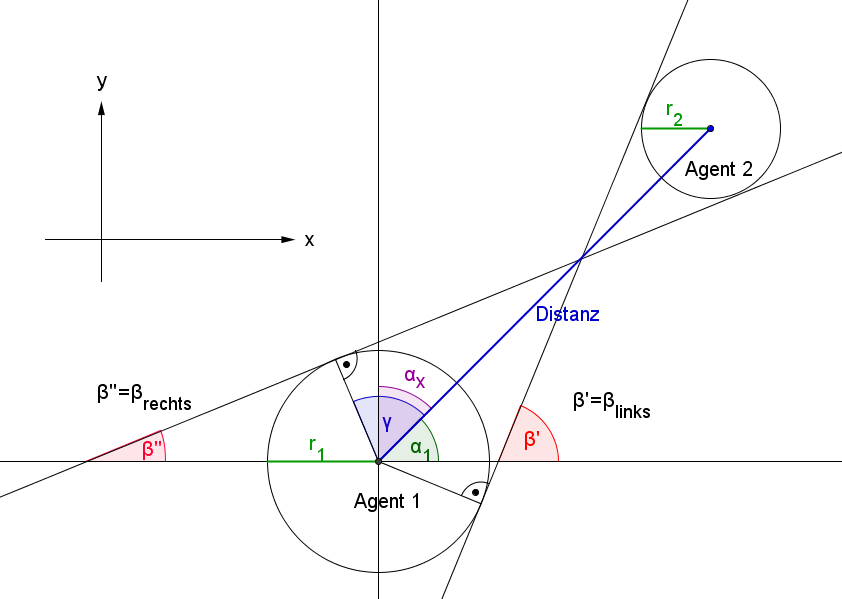
\includegraphics[width=0.80\textwidth]{pictures/beta.PNG}
	\caption{The graph shows the angles and variables used to get $\beta_\y{Links}$ and $\beta_\y{Rechts}$. $\alpha_X$ is the angle between the two agents with respect to the $y$-axis. This depiction was engineered to work also for agents walking the other way.}
	\label{fig:beta}
\end{figure}

\noi For our model, it is crucial to determine where an agent shouldn't go. The function \textit{getBeta.m} returns the angles which describe the interval of angles leading to a collision. A graphical depiction of the situation is given in figure \ref{fig:beta}. The equations (\ref{logik3}) to (\ref{logik5}) were used to get $\beta_\y{Links}$ and $\beta_\y{Rechts}$. They had to be converted into the angles given with respect to $\varphi$, $\beta_{\varphi,\y{ left}}$ and $\beta_{\varphi,\y{ right}}$ as shown in equations (\ref{logik6}) to (\ref{logik7}).
\begin{equation}\label{logik3}
	\gamma = arccos\brac{\frac{r_S}{d}},\ \alpha = arctan\brac{\frac{\Delta y}{\Delta x}}
\end{equation}
\begin{equation}\label{logik4}
	\beta_\y{Links} = \gamma + \alpha - \frac{\pi}{2}
\end{equation}
\begin{equation}\label{logik5}
	\beta_\y{Rechts} = \alpha + \frac{\pi}{2} - \gamma
\end{equation}
\begin{equation}\label{logik6}
  \beta_{\varphi,\y{ left}} = \frac{\pi}{2} - \beta_\y{Links} = \pi - (\gamma + \alpha)
\end{equation}
\begin{equation}\label{logik7}
  \beta_{\varphi,\y{ right}} = \frac{\pi}{2} - \beta_\y{Rechts} = \gamma - \alpha
\end{equation}
\noi This works between agents as well as between agents and the wall agents. Care was taken to engineer a calculation that allows for it to be used for agents walking in both directions.

\subsubsection{Calculation of the interaction with another dynamic agents}
\text{xValuesLogic.m} distinguishes three different cases.
\begin{itemize}
	\item For two crossing agents or if the agent in front of the agent in question is slower, we used equation (\ref{logik1}) to get $x_\y{out}'$. It was also used for two not moving agents, setting $\Delta v$ equal to an arbitrary value given in \texttt{STANDOFF}. This was a quick way to resolve standoffs, although this would eventually turn out to be in its actual form an Achilles heel of the model.
	\begin{equation}\label{logik1}
		x_\y{out}' = \frac{1}{\dis (|x - \alpha_X|)^{\brac{\frac{-\Delta v}{a}}}} = (|x - \alpha_X|)^{\brac{\frac{\Delta v}{a}}},\ \Delta v < 0
	\end{equation}
	\noi All values which correspond to a collision course in $x_\y{out}'$ are set to zero. This also deals with the singularity of equation (\ref{logik1}) as it is set to zero. This is done using the $\beta$-angles shown before. Afterwards, $x_\y{out}'$ is normalized and modificated further using equation (\ref{logik2}).
	\begin{equation}\label{logik2}
		x_\y{out} = x_\y{out}' \cdot \frac{b}{max(x_\y{out}')} \cdot \brac{\frac{r_S}{d}}^c
	\end{equation}
	\noi The variables $a$ (called \texttt{SLOPEFACTOR}), $b$ (\texttt{HEIGHT}) and $c$ (\texttt{REPULSIONAGENT}) have to chosen in a way that the simulation runs smoothly. The term $\frac{b}{max(x_\y{out}')}$ normalized the function to a maximum value $b$ while the term $\brac{\frac{r_S}{d}}^c$ controls that the repulsive influence gets stronger, the closer the two agents get. $c$ is usually chosen to be larger than 1.\\
	For two agents walking the in the same direction, the function given in equation \ref{logik2} is additionally multiplied with the difference in speed $|\delta v|$ in a try to make them avoid standing agents more resolute as it that case $|\delta v|$ would be rather big.\\
	
	\noi If the $x_\y{out}$ given in equation (\ref{logik2}) would be returned, the agent in question would aim to miss the other agent exactly. We thought that this would be too close as in reality, one also leaves a bit of space if possible between each other. Therefore we introduced an offset given as \texttt{WALLANGLEOFFSET} which gives the angle additionally to the $\beta$ angles for which an agent should aim to. To account for this, $x_\y{out}$ is modified with an linear interpolation between the values at $\beta + $\texttt{WALLANGLEOFFSET} and $\beta$ (which was set to zero before).

	\item If the agent in front of the agent in question is faster, a gaussian curve was used with the mean $\alpha_X$ and standard deviation $rS/d$. It is then modified further with $\Delta v$ and \texttt{HEIGHT} to make it a weak influence.
	\item For two agents moving with the same speed, the influence is set to zero by returning a vector of zeros.
\end{itemize}


\subsubsection{Calculation of the interaction with a wall agents}
To avoid hitting the wall, we used a very simple approach. Every angle corresponding to a collision course is set to a negative value accoring to equation (\ref{logik8}).
\begin{equation}\label{logik8}
	x_\y{Out} = x \cdot \frac{a}{d - rS}
\end{equation}
\noi As before for agents, an offset is introduced so the agent in question doesn't just try to avoid the wall-agent but also to leave some buffer space. The offset is also given in \texttt{WALLANGLEOFFSET}, $a$ can be accessed with the constant variable \texttt{WALLFACTOR}. $a$ has to be set negative as otherwise the wall would have an attracting force. To set a good value for this factor $a$ is quite delicate because if it is too low, agents will be stuck in the wall while if it too high, they will never approach the wall even slightly. 

\pagebreak
\subsubsection{Calculating functions in $x$ and transforming them into a polar axis in $\varphi$}
\begin{figure}[h!]
	\centering
		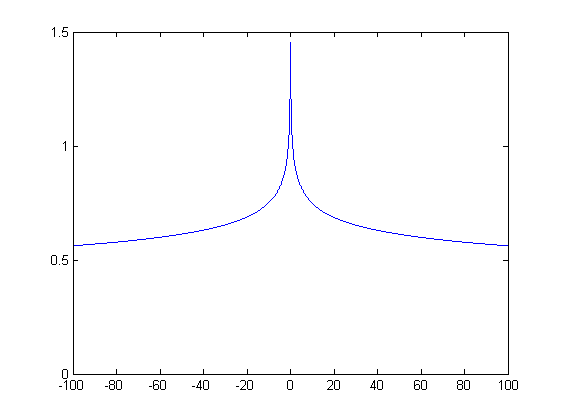
\includegraphics[width=0.40\textwidth]{pictures/Bsp2}
		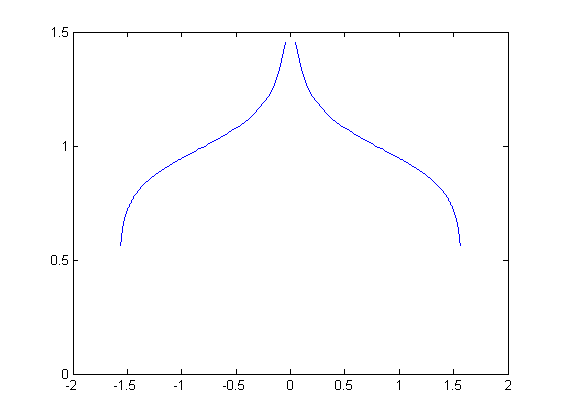
\includegraphics[width=0.40\textwidth]{pictures/Bsp2Angle}
	\caption{Graphical depiction of the function given in equation (\ref{logik1}). In the graphic on the left, the horizontal axis is given in $x$ while in the right graphic the horizontal axis is given in $\varphi$.}
	\label{fig:Bsp2}
\end{figure}

\noi As the functions given above are given in $x$ but the direction to go on is determined in polar values, it needs to be transformed into a $\varphi$ axis. This is done using a vector for $x$ ranging $\pm$ \texttt{XSCOPE} with a step of \texttt{XRES}. Applying the arcustangent on it yields the axis in angular values ($\varphi$). The transforming is done simply by using the $\varphi$ axis instead of the $x$ axis. This is shown in the two figures \ref{fig:Bsp2} and \ref{fig:Bsp2Out}. As those functions are only chosen to show the principle, they were not normalized in height according to the equations mentioned above.\\
\begin{figure}[h!]
	\centering
		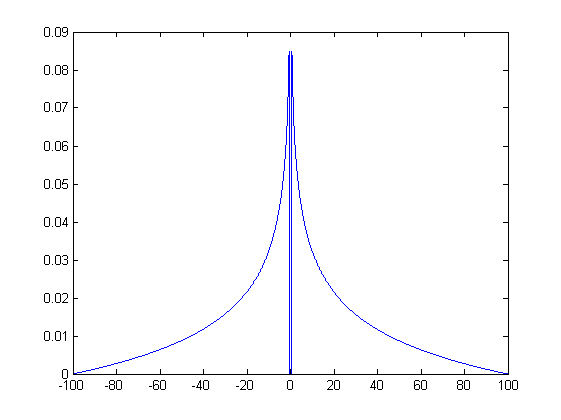
\includegraphics[width=0.40\textwidth]{pictures/Bsp2Out}
		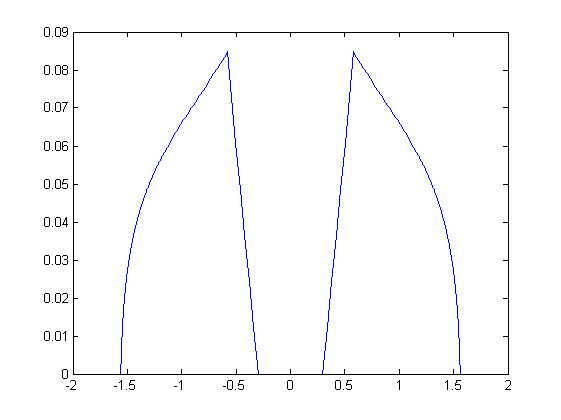
\includegraphics[width=0.40\textwidth]{pictures/Bsp2OutAngle}
	\caption{Graphical depiction of the return values of the function \textit{xValuesLogic.m}. In the graphic on the left, the horizontal axis is given in $x$ while in the right graphic the horizontal axis is given in $\varphi$. $\alpha_X$ was set to 0 corresponding to an other agent directly ahead, $\beta$ was set to $\pm 0.3$ with an offset of $0.25$.}
	\label{fig:Bsp2Out}
\end{figure}

In figure \ref{fig:Bsp2}, the function (\ref{logik1}) is shown graphically in the $x$ as well as $\varphi$ axis. Figure \ref{fig:Bsp2Out} shows the $x_\y{out}$ the function \textit{xValuesLogic.m} returns.



\subsubsection{Graphical example}
This subchapter shall give a visual example of how the logic functions work. Let's consider the situation given in figure \ref{fig:Bsp1}.
\begin{figure}[h!]
	\centering
		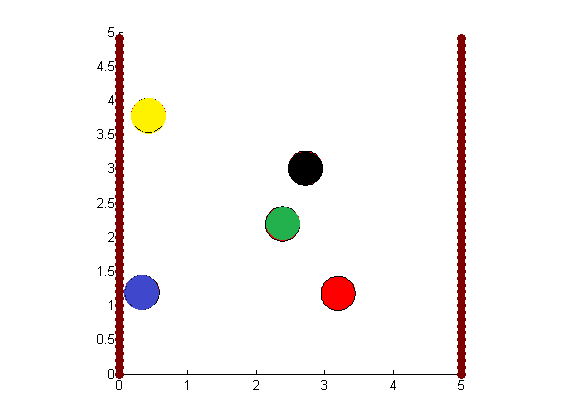
\includegraphics[width=0.45\textwidth]{pictures/Bsp1}
	\caption{Exemplary case used to demonstrate the working principle of the logic functions.}
	\label{fig:Bsp1}
\end{figure}

\noi The blue agent moving up in figure \ref{fig:Bsp1} only sees the influence of the wall. What the blue agent "sees" is given in figure \ref{fig:Bsp1LinksUnten}. The influence of the wall causes the overall function to decrease for all $\varphi$ corresponding to a collision course. The offset causes the overall function to have its maximum $\alpha$ at a positive $\varphi$. This causes the agent to walk in the direction of $\alpha$.\\
\begin{figure}[h!]
	\centering
		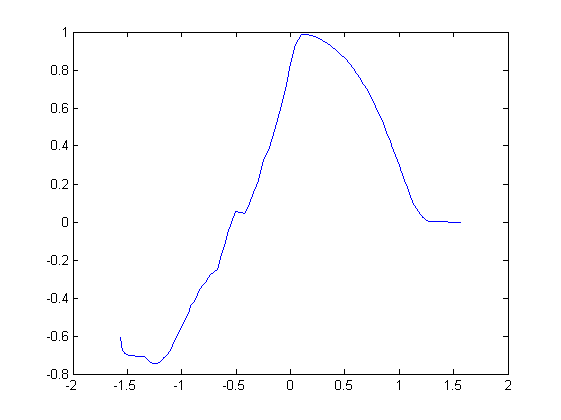
\includegraphics[width=0.4\textwidth]{pictures/Bsp1LinksUnten}
	\caption{Output of all logic functions combined for the blue agent in figure \ref{fig:Bsp1}. Visible is the effect of wall agents on the blue agent as negative values on the left side.}
	\label{fig:Bsp1LinksUnten}
\end{figure}

\noi The green agent moving up sees only the influence of the black agent who is moving down. The effect of that it given in figure \ref{fig:Bsp1Mitte}. The underlying gaussian function can be seen as well as the addition of a modified version of figure \ref{fig:Bsp2Out}, left. The agent will move slightly to the left to avoid hitting the black agent.\\
\begin{figure}[h!]
	\centering
		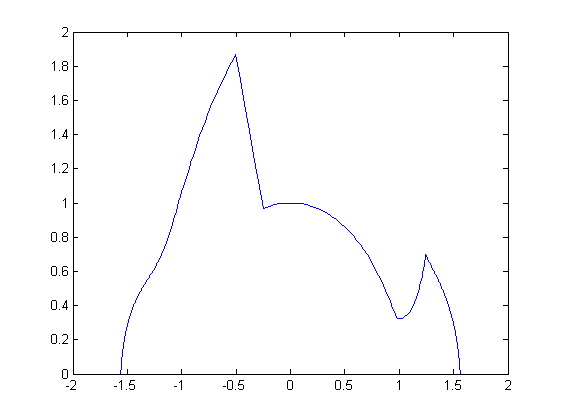
\includegraphics[width=0.40\textwidth]{pictures/Bsp1Mitte}
	\caption{Output of all logic functions combined for the green agent in figure \ref{fig:Bsp1}. Visible is the effect of the oncoming black agent as a superposition on the underlying gaussian curve.}
	\label{fig:Bsp1Mitte}
\end{figure}

\noi The black agent moving down sees the oncoming green and red agent going up. The effect of them is given in figure \ref{fig:Bsp1ObenRechts}. The superposition of two functions onto the underlying gaussion can be seen by the discontinities. The effect of the green agent is stronger as it is nearer to the black agent than the red agent which causes the black agent to go left (looking top-down) in order to avoid hitting the green agent. This shows the dependency of the strength of an agent of the distance.
\begin{figure}[h!]
	\centering
		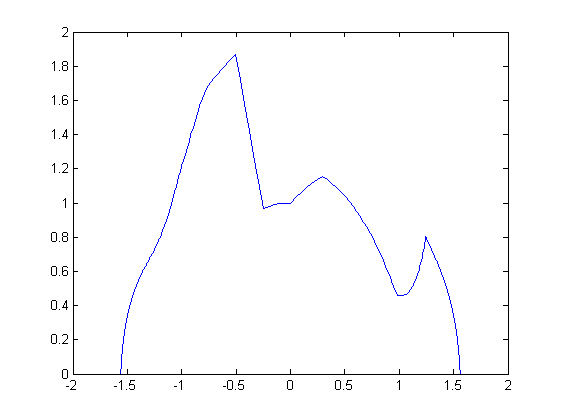
\includegraphics[width=0.40\textwidth]{pictures/Bsp1ObenRechts}
	\caption{Output of all logic functions combined for the black agent in figure \ref{fig:Bsp1}. Visible is the effect of the oncoming green and red agents as superpositions on the underlying gaussian curve. The black agent will move left (from his point of view) to avoid hitting the closer green agent.}
	\label{fig:Bsp1ObenRechts}
\end{figure}


\subsection{Iteration} %Iterationsfunktion und Kollisionsabfragen hier beschreiben. Ebenso die Erschaffung der Agents durch spawn


\clearpage

\subsection{Simplifications}
\begin{itemize}
\item[x] All our agents walk on their own, there are no groups of friends, families etc who stand together as much as possible.
\item[x] The agents are not able to walk backwards, they only can see and walk 90� to each side.
\item[?] All have the same mean speed, size, ??
\item[?] Any other simplifications?
\end{itemize}

\newpage

\section{Performed simulations}
%Experiments

\noi Listed below are the carried out simulations with their most important parameters. For each series of simulations, a brief explanation is given to state the questions which will be looked at with the actual simulation series.\\
All parameters can be found in the corresponding logfiles. Usually only one parameter was varied while all others were kept constant. We chose a mean radius for the agents of 0.25 meters with a standard deviation of 0.03 meters. A mean velocity of 1.5 meters per second was chosen with a rather large standard deviation of 0.25 meters per second.\\
It should be noted that we usually used high people flux densities since we wanted to test the model under stress conditions. Therefore we expected a considerable amount of failure in the examined situations.

\subsection{Influence of different pedestrian flux densities}
To check the influence of different densities on our model, we ran the simulation with the density combinations 0.4/0.4, 0.4/0.6, 0.4/0.8, 0.4/1.0, 0.6/0.6, 0.6/0.8, 0.6/1.0, 0.8/0.8, 0.8/1.0 and 1.0/1.0. The first number represents the value chosen for \texttt{DENSITYDOWN}, the second for \texttt{DENSITYUP}. We didn't run the inverted combinations due to the situation's symmetry. The simulations were repeated with three different seeds each, 51, 71 and 91. A high value for \texttt{DISPERSIONFACTOR} of 1.0 was chosen which corresponds to people having a strong tendency to try to overtake slow agents. All simulations were run for 120 seconds.

\subsection{Influence of overtaking or lane formation on the success of the model}
It soon became clear to us that the parameter \texttt{DISPERSIONFACTOR} would be absolutely crucial if one wants to force the model to succeed. A negative value encourages the agents to form lanes while a positive value encourages them to try finding their own way. In order to investigate this property, specially with the dilemma of personal vs. group success in mind, we ran a simulation series where we incremented the \texttt{DISPERSIONFACTOR} from -0.2 to 1 each time by 0.1. A high density flux of 1 person per second on both sides was used to test the model in a stress situation. This was done for three different seeds each, 51, 151 and 351. All simulations were run for 120 seconds.

\subsection{Influence of the radius of sight of an agent}
The constant variable \texttt{INFLUENCESPHERE} determines the radius of the semi-circle in which the agent considers other agents around him. With flux densities of 1.0 each and a \texttt{DISPERSIONFACTOR} of 0.7, the \texttt{INFLUENCESPHERE} was tested using the values 1.5, 2.0, 2.5 and 3.0 (in meters). This was done for three seeds each, 51, 77 and 151. All simulations were run for 120 seconds.

\subsection{Influence of the hallway width on the success of the simulation}
To account for the influence of the width of the hallway on the success of the simulation, we did a simulation series with different widths. The tested widths were 2.2, 2.5, 2.8, 3 and 3.5 meters. A high density flux of 1 person per second on both sides was used with a \texttt{DISPERSIONFACTOR} of 0.75 corresponding to a high number of overtaking attempts. The simulations were repeated with the seeds 51, 77 and 151 each. All simulations were run for 100 seconds.

\subsection{Simulating measurements of the main station Zurich}
Saturday, Nov 17th, we did some quick measurements right at Zurich main station to have some data we could try to compare. Two measurements were taken, only some minutes lay between these, that was when we measured the length and breadth of our corridor. The measurements were:
\begin{enumerate}
\item The "boring" measurement: During 2 minutes, 14 pedestrians headed towards tracks 3-18, and 20 pedestrians directed towards tram station "Bahnhofsquai". No problems at all, very fluently.
\item The "crowded" measurement: During 2 minutes, 41 pedestrians headed towards tracks 3-18, and 33 pedestrians directed towards tram station "Bahnhofsquai". People got stuck, ran into each other, and had to walk stop-and-go-like for some moments.
\end{enumerate}
\noi In order to simulate this, we used values of 0.12 (up) and 0.17 (down) as flux densities for the first measurement, the second measurement was simulated with flux densities of 0.34 (up) and 0.275 (down). In all cases, a \texttt{DISPERSIONFACTOR} of 0.7 was chosen. These values represent the measured flux densities.\\
To get also something like a rush hour, we simulated a situation with approximately double flux densities than in the "crowded" measurement, namely with 0.6 (up) and 0.5 (down). All simulations were run for 180 seconds.

\subsection{Simulation of a big inequality in the flux densities}
This series was designed to test how a small number of people walking up would react to a big number of walking down. To test this, the flux density walking down was kept constant at 1.0 while the flux density of people walking up was varied with the values 0.2, 0.3 and 0.4. \texttt{DISPERSIONFACTOR} was again set to 0.7 with an iteration time of 180 seconds. The used seeds were 51, 91 and 113.\\

\noi The simulations were carried out with \textsc{MATLAB R2011a} on a \textsc{HP EliteBook 8400p} (Intel Core i7 CPU M620 @ 2.67 GHz) with a windows 7 professional operating system.


\newpage

\section{Simulation Results and Discussion}
%ResultsAndDiscussion

%vgl. auch Introduction and Motivation
%vgl. auch Abstract
%had to drop some of our goals because we wanted to build everything up on our own.
%erw�hnen (zB bei discussion), dass Imagine und Nordshizzle w�hrend Christkindmarkt jetzt die Tische/St�hle aus dem Weg r�umen!
%beachten, dass wir mit "jeder l�uft alleine" statt "es gibt auch Gruppen von Leuten" eine ziemlich starke Einschr�nkung/Vereinfachung vorgenommen haben!

%Discussion
\subsection{Goals}
First, let's have a look at what our goals were. We planned to have a look at the pedestrian flux, how it can be improved and jammings be avoided. We furthermore wanted to have a closer look to what happens during rush-hours and in a situation when much more people are moving in one direction than in the other.\\
On the agent-based side of our model, we wanted to analyze the influence of aggressive fast people in a rush, slowly moving obstacles (eg. mothers with baby buggies) and the influence of drunkard (more or less randomized walking) on the pedestrian flux.\\
If everything went well, we also wanted to implement a static obstacle and see what happens. As a reminder before the discussion of the results, our fundamental research questions were:
\begin{itemize}
\item How does the simulation behave in the following situations: rush hour, with obstacle, with very slow/fast agents, random path agent (drunkard)? Does it run smoothly or will ther be jams?
\item How will our implementation of a rudimentary kind of "`thinking ahead"' affect the simulation? Will it work good or bad? Can we compare it to other implementations?
\item Are there any group dynamics evolving as lane or group formation?
\end{itemize}

\subsection{General achievements}
As soon as we started programming we realized there was a major point of importance about this work we all were aware of, but had forgot to put it in the project proposal. We all did not want to start with an already known program or existing algorithms, but build something "new". So we started off creating our logic function that would allow the agents to avoid crashing into other agents and not working with repulsive forces as for example Helbing (Quelle angeben, ist das �lteste Paper) did.\\
Quite proudly, we can now say we managed to do this. Our idea of the agents "thinking ahead" by consulting where other agents are and not just being pushed around by repulsive forces worked.\\
We now are able to play with lots of input variables, the most important being number of agents entering the corridor per time and the agents' characteristics as size, speed and lots more.\\
A nice thing we built but did not originally plan to is that we planned to and did research on the sitation as explained earlier in the long, narrow corridor in Zurich mainstation. But in our simulation, one can also change dimensions as length and shape of the walls easily.\\

\noi We therefore decided to make first of all sure that the model works and what are its operating parameters. This meant that we had to drop a lot of our former goals because we did not want to carry on with a faulty model. Therefore we have included some results that were not included in our first questions we set out to answer in the beginning.\\
On the downside of this, we dropped the investigation into the behaviour of the pedestrian flux when exposed to aggressive, slow or random people. Even though these situations were not simulated, the functionality to introduce them without much work was implemented into the model as they were considered when we built our model.

\subsection{Results from the simulation series}
\subsubsection{Influence of different pedestrian flux densities}
% Influence of different pedestrian flux densities

\noi For this experiment we monitored the total agents count as an indicator for jams. This number was then scaled by the combined flux densities to give comparable results which can be found in figure \ref{fig:AAllAveragesScaled}.\\
\begin{figure}[h!]
	\centering
		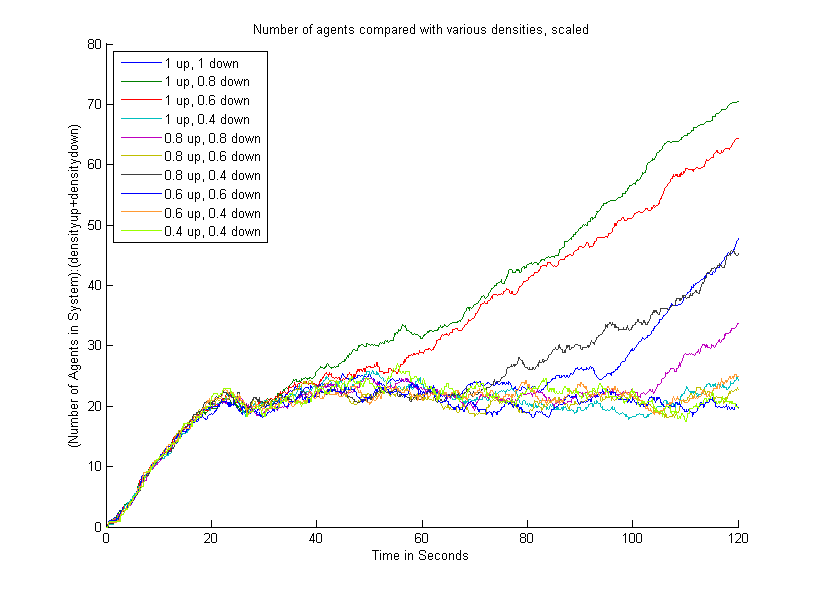
\includegraphics[width=0.80\textwidth]{pictures/AAllAveragesScaled.png}
	\caption{The scaled total number of agents in the system for various combinations of flux densities with respect to time. The used flux densities are given in the graph legend. As soon as the total number of agents runs away, a jam has formed. The mean over three simulations with different seeds was taken for each case. As expected high flux densities caused massive jams.}
	\label{fig:AAllAveragesScaled}
\end{figure}

\noi With the highest flux densities used in the simulations, the jam formation was very fast. It is interesting that 0.6/0.6, 0.8/0.4 and 0.8/0.8 also caused jams within the observed time frame, specially since 1/0.4 didn't jam.\\
Our model seems not to be able to cope well with that many people. There should be more simulations with different seeds to get a better statistic.\\

\begin{figure}[h!]
	\centering
		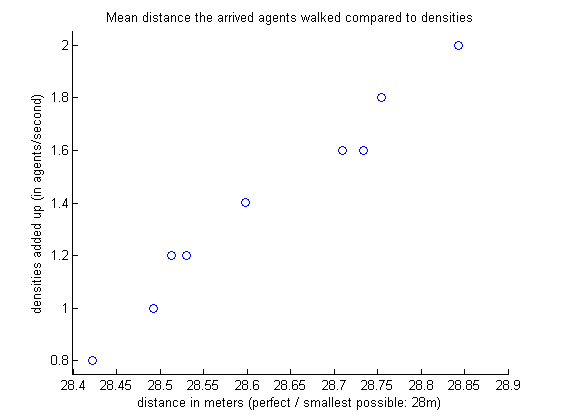
\includegraphics[width=0.49\textwidth]{pictures/AMeanDistancesCompared.png}
		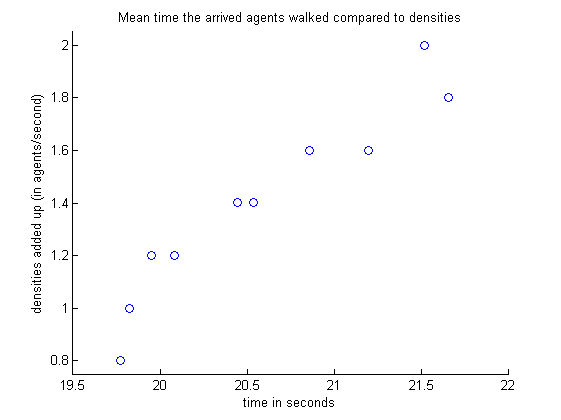
\includegraphics[width=0.49\textwidth]{pictures/AMeanTimeCompared.png}
	\caption{Graphs of the mean covered distance and mean time spent during the simulation for all agents who reached their destruction line compared with the combined flux densities used. As expected, for high flux densities the agents have to cover longer distances and spend more time as they have to avoid colliding with other agents.}
	\label{fig:ACompared}
\end{figure}

\noi Given in figure \ref{fig:ACompared} are the mean covered distance and mean time spent during the simulation for all agents who reached their destruction line compared with the combined flux densities used. As would be expected, the agents had to cover a longer distance and spend more time in the simulation as they had to avoid collisions with other agents.\\
These variables were monitored to analyze whether they give a good description of the model and to ensure that we got results that run within the same expectations as in reality. But as they only take the values of those agents that have left the simulation, they may have a decreased significance when jams occur and are not at all able to tell whether a jam has occured or not.




\subsubsection{Influence of overtaking or lane formation on the success of the model}
% Influence of overtaking or lane formation on the success of the model

\begin{figure}[h!]
	\centering
		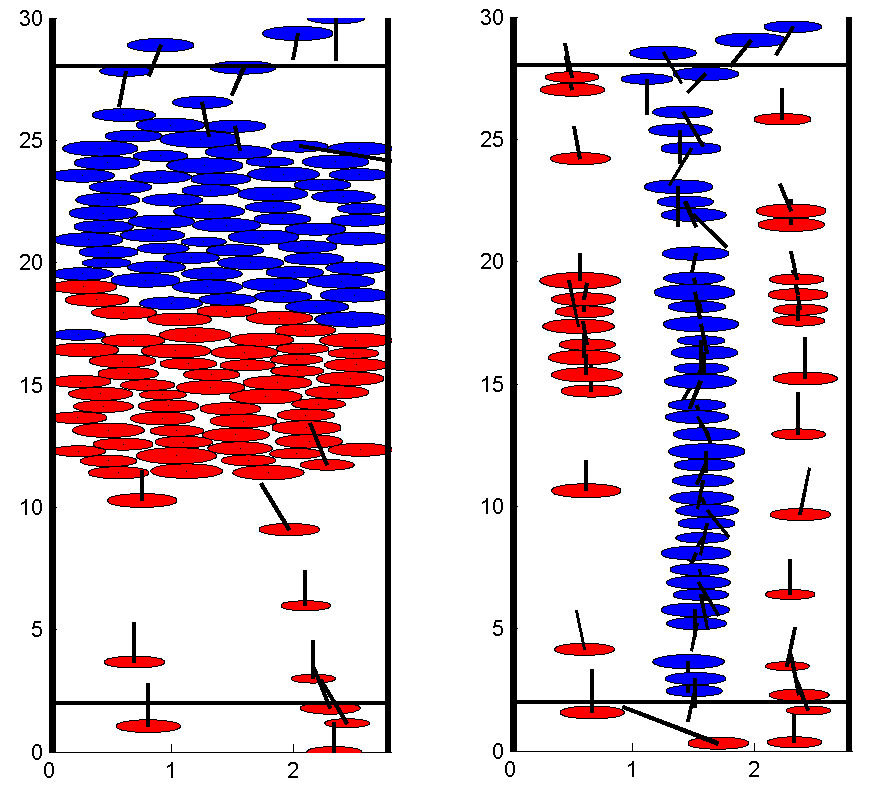
\includegraphics[width=0.8\textwidth]{pictures/ex2picture.png}
	\caption{Exemplary pictures of our simulation after a simulation time of 120 seconds. The right one was run with a \texttt{DISPERSIONFACTOR} of 1 while the left picture has one of 0.1. The jaming to the left and the lane formation to the right can be seen.}
	\label{fig:ex2picture}
\end{figure}

\noi Some examples of how our simulation did look like after a simulation time of 120 second are given in \ref{fig:ex2picture}.\\

\noi In figure \ref{fig:AAllInOne} all collected data is consensed into one graph which was visualized in two ways. Another representation of the same data is given in the appendix in figure \ref{fig:ADistanceSeedsFactors} (page \pageref{fig:ADistanceSeedsFactors}). They correlate the average distance covered per agent per iteration step with the simulation time. There were two expectations: As soon as a jam starts to form, this variable should decrease quite fast. An lane formation should be detectable as most agents will not be able to walk with their maximum speed so the average distance per agent per timestep should be significantly below the mean value given by $\bar{d} = \Delta t \cdot \bar{v}$, the product of \texttt{DELTAT} with \texttt{MEANSPEED}.\\

\begin{figure}[h!]
	\centering
		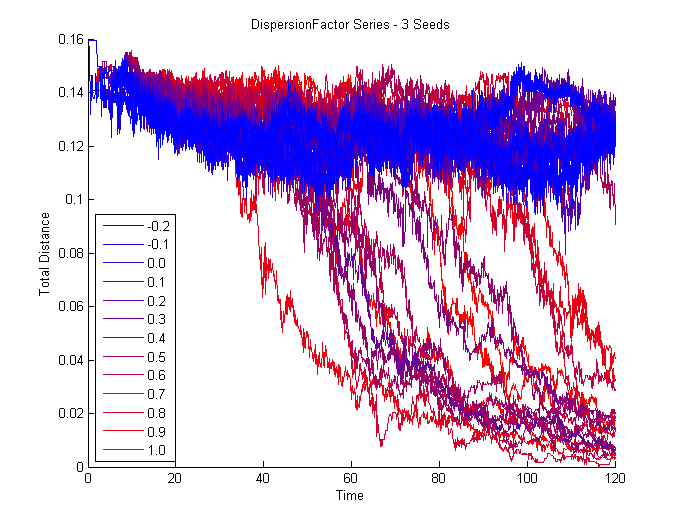
\includegraphics[width=0.49\textwidth]{pictures/AAllInOneColorsBlue.png}
		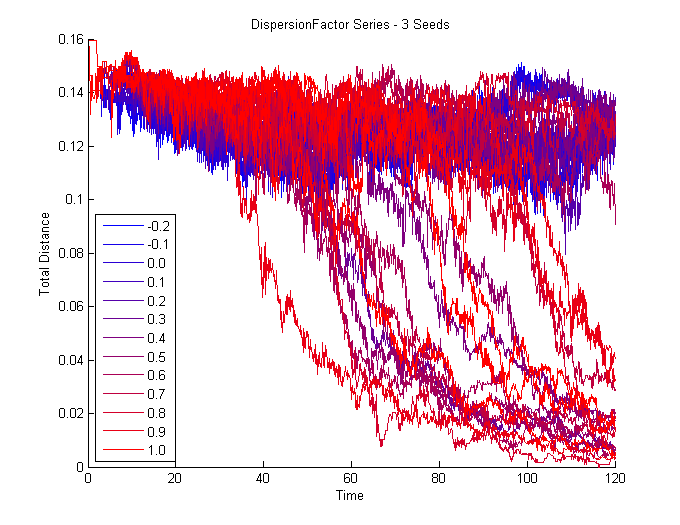
\includegraphics[width=0.49\textwidth]{pictures/AAllInOneColorsRed.png}
	\caption{Graph of the average covered distance per agent present in the simulation per step as a function of time. The more blueish the color is, the stronger was the agents tendency to form lanes while the more reddish the color is, the stronger was the agents tendency to try to overtake slow agents. In the left graph the more blue lines are highlighted while in the right graph the more red lines are highlighted. Although the red lines representing "greedy" agents cope well at the very start, the usually lead to a jam very quickly.}
	\label{fig:AAllInOne}
\end{figure}

\noi Given the two graphs, it is striking that the majority of the simulations represented by reddish lines representing high values of \texttt{DISPERSIONFACTOR} fail during the observed time frame. At rare occasion though the simulation was successful even with a relatively high \texttt{DISPERSIONFACTOR}.\\
On the other side, there was always lane formation for a \texttt{DISPERSIONFACTOR} below 0.4, represented by the more blueish lines which ultimately resultet mostly in successful simulations without jamming.\\
The lane formation can be seen quite clearly in the graphs given in figure \ref{fig:AAllInOne}. The reddish lines try to keep the mean distance at almost all cost, this is visible in the initial height of the reddish lines. In contrast, the blueish lines quickly fall down by about 0.02 meters per agent per iteration step which is a precise indication of lane formation. But in the long run, the best reddish line performed about equally well as most blueish lanes, indicating that in crowded situations like this, cooperation between agents in the form of line formation is not worse in peformance as the best egoistic approach but succeeds way more often.\\

\noi It seems that the forced lane formation was a successful way to resolve the problem of jaming. It also highlights the importance of cooperation and the sensitivity of our model towards this parameter.



\subsubsection{Influence of the radius of sight of an agent}
% Influence of the radius of sight of an agent

\noi The constant variable INFLUENCESPHERE determines the radius of the semi-circle in which the agent considers other agents around him. With flux densities of 1.0 each and a DISPERSIONFACTOR of 0.7, the INFLUENCESPHERE was tested using the values 1.5, 2.0, 2.5 and 3.0 (in meters). This was done for three seeds each, 51, 77 and 151. All simulations were run for 120 seconds.

\begin{figure}[h!]
	\centering
		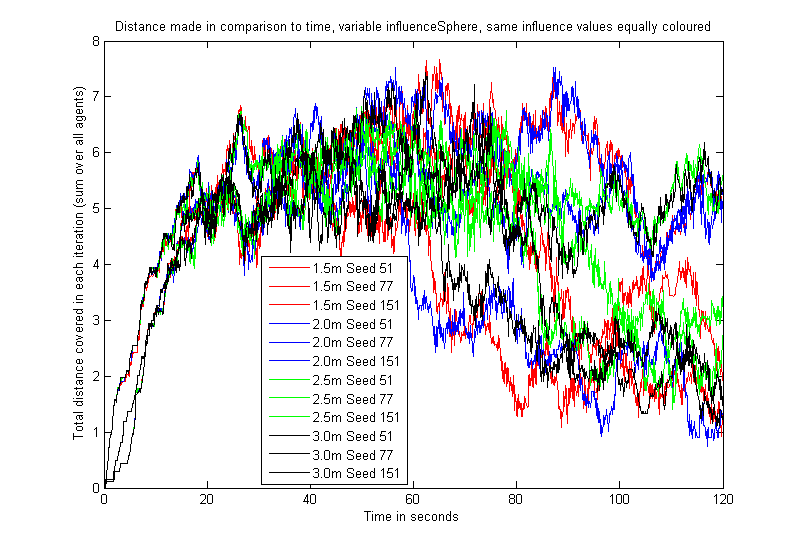
\includegraphics[width=0.80\textwidth]{../../code/sim/Influence/ATotalDistanceInfluencesColoured.png}
	\caption{This plot shows the total distance covered by all agents in the system for different influence sphere radii and seeds in dependence of the simulation time. This distance decreases rapidly when a jam starts. To show the total distance's dependence on the influence sphere radius, each seed to a certain radius was coloured equally. Only these radii were varied in these simulations. One can see here that there is no clear dependence of the radii to the total distance as for every radius except 1.5m there are seeds that work and seeds that don't, which means they had jams.}
	\label{fig:InfluencesColoured}
\end{figure}

First of all, the dependency between the influence sphere's radius and the total distance walked by all agents has to be evaluated. As shown in figure \ref{fig:InfluencesColoured}, neither dependencies nor tendencies can be seen clearly, as of every radius, some seeds worked well where other simulations for the same seed jammed.

\begin{figure}[h!]
	\centering
		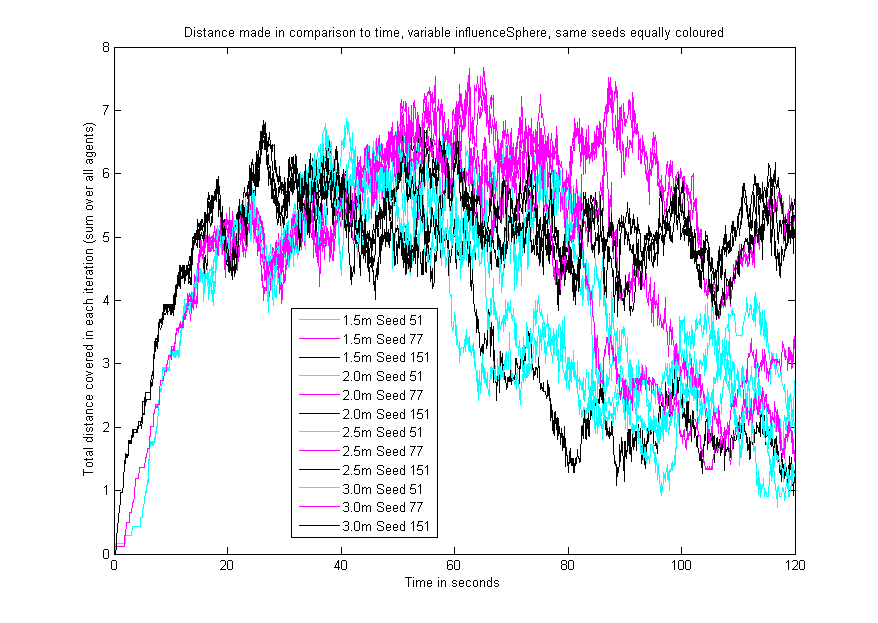
\includegraphics[width=0.80\textwidth]{../../code/sim/Width/ATotalDistanceSeedsColoured.png}
	\caption{This plot shows the total distance covered by all agents in the system for different influence sphere radii and seeds in dependence of the simulation time. This distance decreases rapidly when a jam starts. To show the total distance's dependence on the seed, each radius to a certain seed was coloured equally. Only these radii were varied in these simulations. One can see here that whether a simulation jams or not seems to depend on the seed, as the seed 51 simulations all jammed independent of the radius, and for the other two seeds, there was only one radius that was different.}
	\label{fig:SeedsColoured}
\end{figure}

Next, there maybe is a depedence between the success of a simulation and the seed which would explain why no clear tendencies for the radii was observed in figure \ref{fig:InfluencesColoured}. So, in \ref{fig:SeedsColoured}, the same seeds were coloured equally, which showed much more of a tendency: A seed seems to have the property that it will most likely jam or not: seed 51 caused jams for every radius, where seed 77 and seed 151 produced a similar result except for outliers.

\begin{figure}[h!]
	\centering
		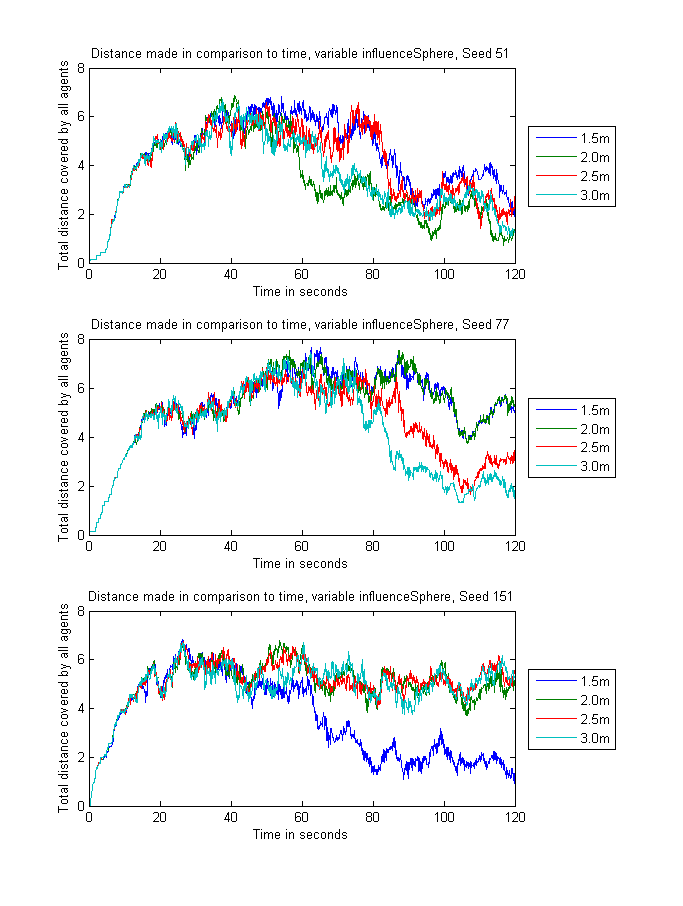
\includegraphics[width=0.80\textwidth]{../../code/sim/Width/ADistancesPerSeeds.png}
	\caption{This plot shows the total distance covered by all agents in the system for different influence sphere radii and seeds in dependence of the simulation time. This distance decreases rapidly when a jam starts. To investigate the radius' dependence on the total distance, the total plot was split up into three parts, each containing all simulations for one seed. Only these radii were varied in these simulations. One can see here that in seed 51, every simulation jammed independently of the radius. In seed 77, the larger radii jammed, on the other hand only the small radius crashed in seed 151.}
	\label{fig:SeedsOverview}
\end{figure}

To investigate this further, the plot was now split up into 3 subplots, one for each seed as figure \ref{fig:SeedsOverview} shows. Again, this seems to show some dependency as assumed in figure \ref{fig:SeedsColoured}, but this could also be coincidence.\\
Here, no dependency can be seen because with seed 51, every single simulation will cause jams. Seed 151 shows what one could expect to see: For a small influence sphere radius, a jam pops up. But seed 77 shows the exact opposite of this as here, the larger influence radii caused jams. So neither dependence nor tendency between influence sphere radius and total distance walked can be observed.

%Discussion
As already seen in chapter $hier verweis zur resultate-section von dieser serie einf�gen$, neither dependence nor tendency between influence sphere radius and total distance walked can be observed because there were opposing trends. Seed 151 showed what we expected to see: For a small influence radius, a jam popped up where for larger radii it didn't. On the other hand, seed 77 showed the exact opposite: only the large radii caused jams.\\
This leads us to think that coicidence played a main role here and shows us another thing: In our formulas weighing the influence of other agents on a specific agents, the weights are too big for very close agents in comparison to agents in a larger distance. This explains why larger radii didn't show the expected results: the additional influence of those agents was too little to matter. The assumption that out weighing function is not perfect can also be observed in any simulation: The agents walk straight forwards to each other for a long time and avoid each other only when they are very close to each other and not from a few meters ahead.


\subsubsection{Influence of the hallway width on the success of the simulation}
% Influence of the hallway width on the success of the simulation




\subsubsection{Simulating measurements of the main station Zurich}
% Simulating measurements of the main station Zurich

\noi The experiments were only analyzed visually by judging how well our model could cope with the given task and how it compared to the real observations. In figure \ref{fig:ex5picture}, one final situation for each run is given as an example.\\

\begin{figure}[h!]
	\centering
		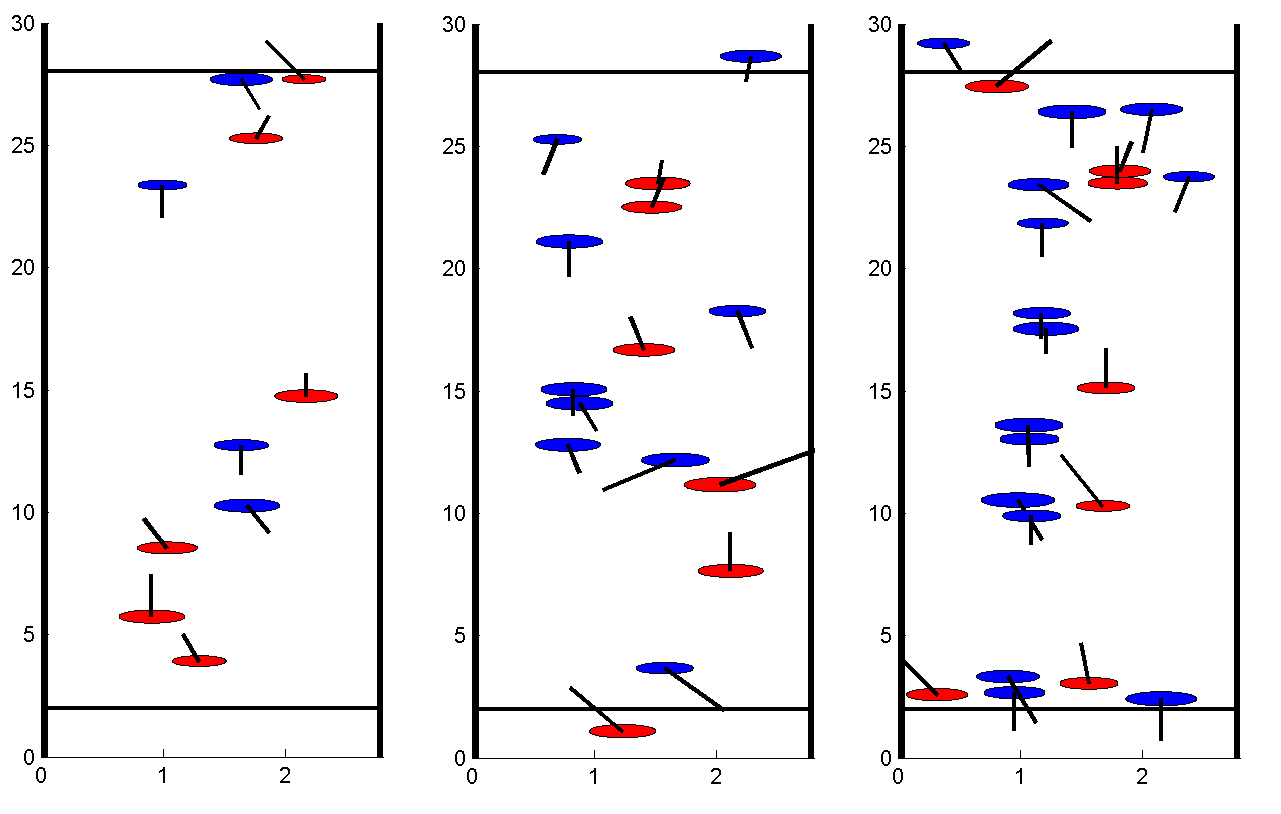
\includegraphics[width=0.90\textwidth]{pictures/ex5picture.png}
	\caption{Exemplary pictures for the simulation of the long narrow hallway in the Zurich main station. Red agents are walking up and blue down, the black line denotes the actual velocity vector with its angle and length. The left was done with flux densities of 0.12/0.17, the middle with 0.34/0.275 and the right with 0.6/0.5 after a simulation time of 180 seconds. In all investigated situations, the agents managed to cross the hallway without significant hindrance from other agents.}
	\label{fig:ex5picture}
\end{figure}

\noi For the first simulation series with a low people flux, the agents had no problems and could avoid collisions/walking into each other easily. This is in accordance with the observations.\\

\noi For the second simulation series with a medium people flux, the agents had little problems crossing the hallway. The stop-and-go of the observation was only rarely seen, suggesting that the logic behind our model is actually quite good.\\

\noi In the third simulation series with a high people flux, the agents had to stop sometimes while getting on the other side. But overall they could cope quite well with the task and the frequency of agents bumping into each other was quite slow and definitely in the same range as in real situations. Sometimes a small lane formation could be observed.\\

\noi We can say that our simulation worked well on the measured quantities. Of course, in reality, when jams start, there will be more side effects as people pushing, turning around, or trying to walk another way, but for a straightforward walk, our simulations mirrors the reality nicely.


\subsubsection{Simulation of a big inequality in the flux densities}
% Simulation of a big inequality in the flux densities

\begin{figure}[h!]
	\centering
		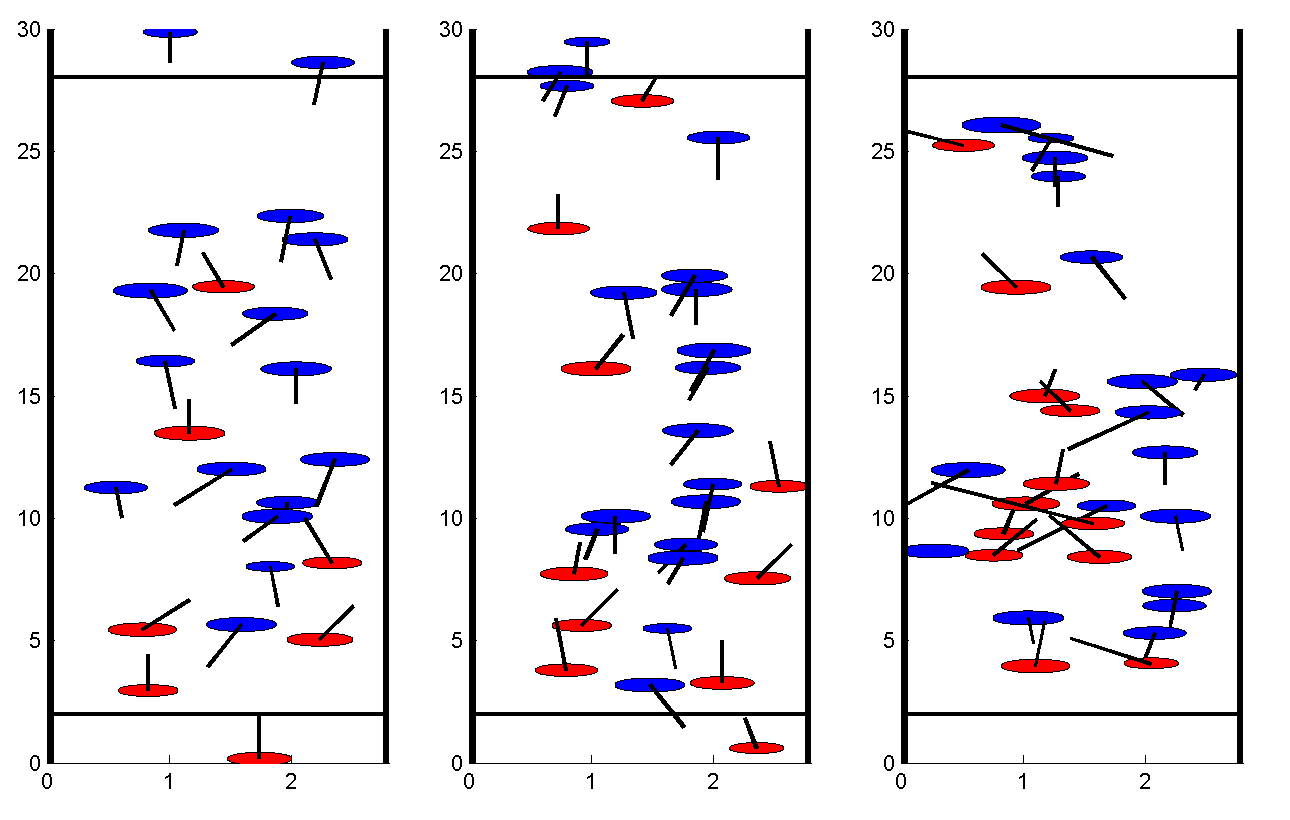
\includegraphics[width=0.85\textwidth]{pictures/ex6picture.png}
	\caption{Exemplary pictures for the simulation of the long narrow hallway in the Zurich main station with highly unbalanced flux densities. Red agents are walking up and blue down, the black line denotes the actual velocity vector with its angle and length. The one on the left was done with flux densities of 1.0/0.2, the one in the middle with 1.0/0.3 and the one on the right with 1.0/0.4 after a simulation time of 180 seconds. The red agents (minority) were wandering about quite strong and usually formed small lanes.}
	\label{fig:ex6picture}
\end{figure}

\noi The experiments were only analyzed visually by judging how well our model could cope with the given task. Some exemplary pictures are given in figure \ref{fig:ex6picture}.\\

\noi For the densities 0.2/1 used in the first series, the overall success was satisfying. The agents walking up (red, minority) were wandering about quite strong due to all the oncoming blue agents. But even though the blue outnumbered the red agents 1:4, the red agents stopped very rarely.\\

\noi In the case of the densities being 0.3/1, the results were quite similar with those obtained by 0.2/1. But the tendency for the red agents to walk in lanes or small groups increased clearly, probably because there are more red agents which are shuffled together by the big number of blue agents trying to stomp their way through.\\
\begin{figure}[h!]
	\centering
		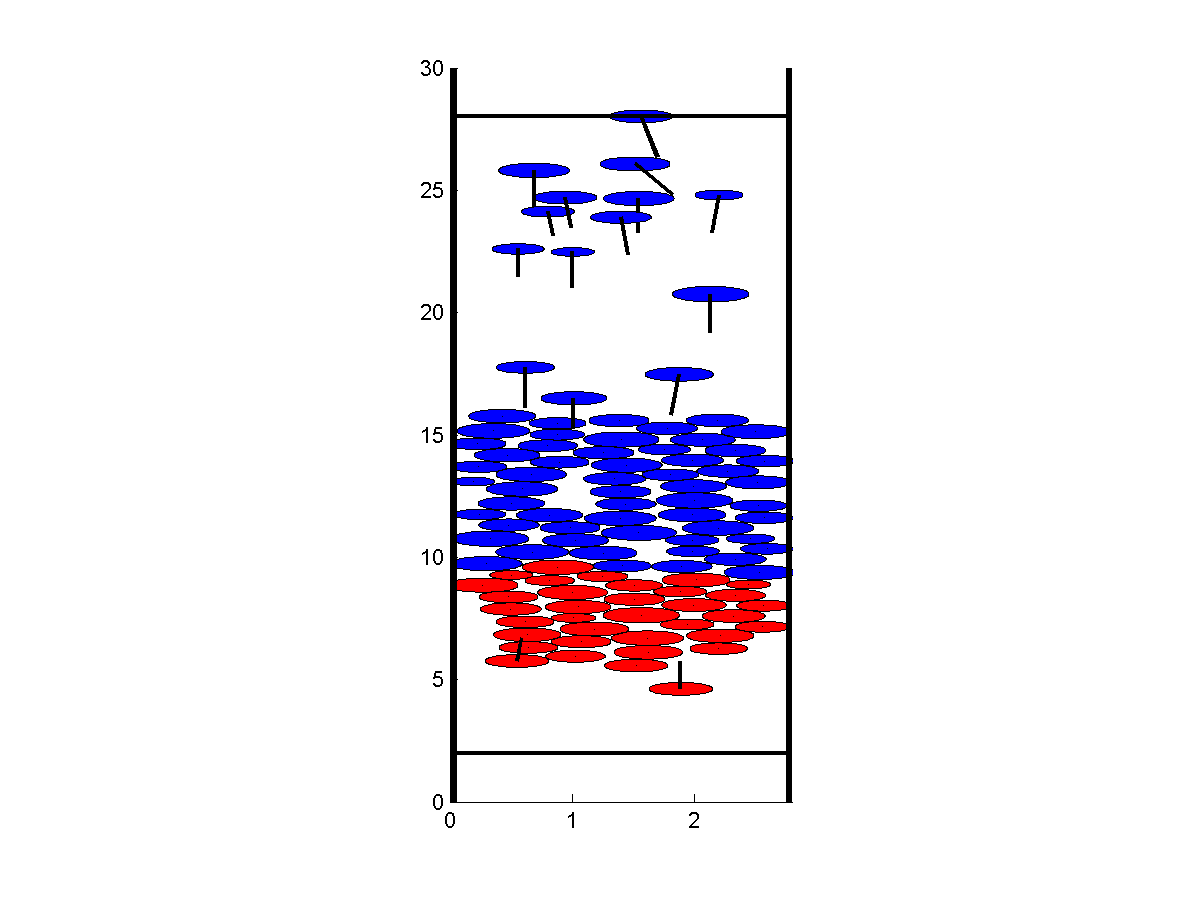
\includegraphics[width=0.90\textwidth]{pictures/up1down04seed51.png}
	\caption{Exemplary pictures for a massive jam in our model. Red agents are trying walking up and blue down, the black line denotes the actual velocity vector with its angle and length. Parameters were flux densities 0.4/1 with a seed of 51. Our model has no way to resolve a jam like that.}
	\label{fig:up1down03seed51}
\end{figure}

\noi For the last considered case, the simulation failed in one case after approximatly 140 seconds (seed 51). The situation after 180 seconds is given in figure \ref{fig:up1down03seed51} as a classical example of how a jam looks like in our model. Before that and in the other two simulations, the red agents formed lanes and little groups very frequently as a way to not always get tossed over the whole width.\\
But the failure suggests that we reached about the limit which can be modelled with our simulation.\\

\noi To sum up, we can say that what we expected could be observed. Anyone who ever went against the tide, for example when people debark a train or bus, knows that advancement is hard to reach. This effect of slowing down and flocking together with other people who try to walk the same way popped up nicely.\\


\subsection{Discussion}
\subsubsection{Simulations}
Overall, we were quite pleased with the results we got from our simulations as they mostly fulfilled our expectations. We could underscore the importance of the choice of a good set of parameters for our model to succeed. It is also possible, as in the case of \texttt{DISPFACTOR}, to change the result very drastically.\\
To address the question whether our model is a good description of the reality even if it cannot descide on itself whether it should start something like a cooperative mode including lane formation or adapt an egoistic approach, we would like to state that the model is only as intelligent as the one who uses it. We leave it to the user of the simulation to set reasonable (and therefore also realistic) values for the global parameters which should match the situation one would like to research.\\

\noi The main simulations concerning the modelling of an actual situation was very satisfying as it performed at least as good as reality. A criticism onto our implementation of the main station in Zurich could be that the flux of people arriving is always kept constant. People familiar with the main station in Zurich would know that there is a pedestrian traffic light just in from of the Burger King, therefore the simulation should probably be adapted to allowing intermittent people spawning with different people flux densities just after the red or green light at the traffic light.\\

\noi It should be highlighted that we saw a big overall performance improvement once we introduced the preference for lane formation. This can be interpreted as implementing a social norm which states that one should back down a little bit from the egoistic main goal of crossing as fast as possible but work together in order to get an acceptable result for everyone.


\subsubsection{Discussion on various implementational issues}
As we created and implemented our model from scratch, there are obviously some undealt issues that would need some refinement if one wants an even better performance of the simulation as such.\\

\begin{figure}[h!]
	\centering
		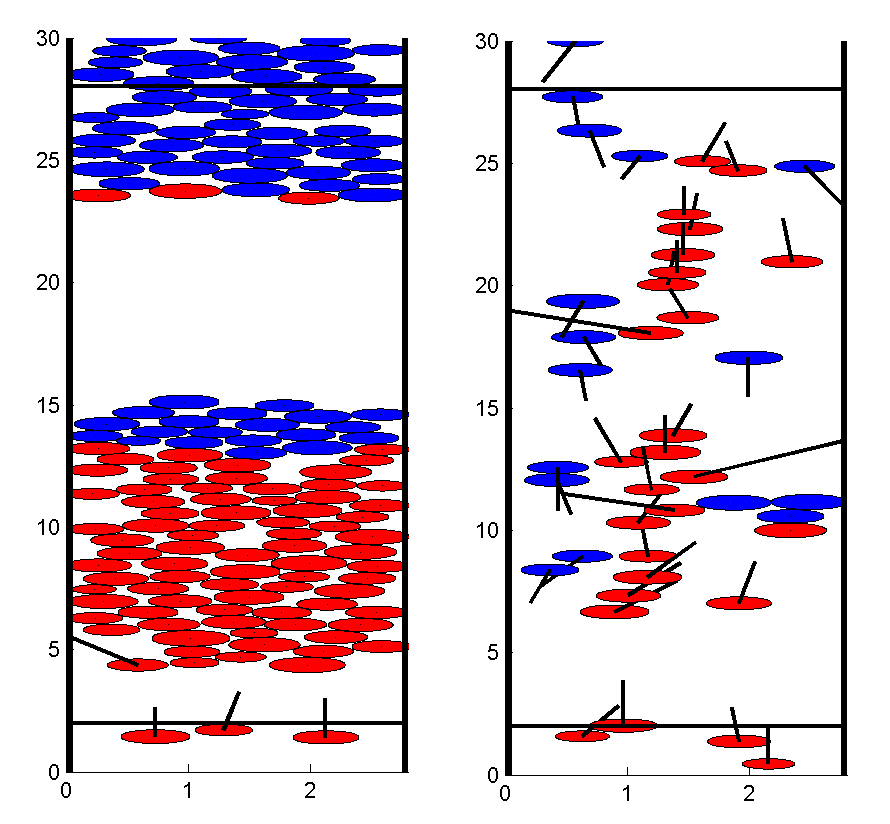
\includegraphics[width=0.90\textwidth]{pictures/exFails}
	\caption{Graphical examples of instructive failures. Graphs were taken from the simulation series to test \texttt{DISPERSIONFACTOR}. In the left graph, we have in the top region the unrealistic situation where three agents block the whole hallway. On the right the earliest stage of a jam is visible with the three blue and one red agent standing in the middle at the right wall.}
	\label{fig:exFails}
\end{figure}

\noi Probably the most important issue of all would be the need of implementing a smarter way to resolve standoffs or detect them earlier. We reckon that a good implementation of this should prove to be rather difficult as one has to distinguish between various cases with various ways to resolve them. This is visualized in figure \ref{fig:exFails} in the right graph. As soon as two (or more) agents totally immobilize each other, the are prone to form a jam.\\
One would probably have to introduce walking backwards to resolve these situations. The effect of not being able to walk backwards is given in figure \ref{fig:exFails} in the left graph on the top in a very instructive way. Three red agents were able to totally freeze the simulation at the top, something that would never happen in reality.\\
Another advantage of a good implementation would be that the runtime on the machine would not explode as it does with the current implementation as soon as a jam has formed. This is rooted in the consideration that all agents within a certain radius shall be considered. Then the logical routine would go over a lot of other agents, even though the agent will not be able to move anyway as he is stuck in a jam.\\

\noi We used to different axis, a $x$- and a $\varphi$-axis as we thought this would make it significantly easier to model various aspects without the trouble of doing the transformation on paper and only use the $\varphi$-axis all the way. Also all angular values had to be discretized to their closest values the $\varphi$-axis has, which was done with the function \textit{closest.m}. This works fine as long as the simulation runs smoothly, but as soon as a jam was formed, the number of calls of \textit{closest.m} exploded. In one case, it was called over 2 million times for 1200 iteration steps in a simulation that had a matlab runtime of about 2 hours (with 4 Matlab instances running parallel).\\

\noi It rarely happens during a simulation that an agent is in an impossible position. This is determined in the collision detection because the first of all calculated points is the position the agent stands on before moving. This was easier to implement and probably not significantly worse in system runtime than excluding it. In rare occasions, the collision detection determines that the agent could not stand at its actual position. We think that this happens due to some small roundoff errors or other computational mistakes.\\
If the agent is at an impossible position, its position would freeze and cause everything around him not to work properly anymore. We could not think of an effective algorithm to resolve these conflicts because they would probably involve setting back the simulation by some iteration steps and simply deleted the agent.\\
We knew that it was not an elegant solution but could settle on the argument that the simulation would otherwise crash. And as the freuency of this occurence is really small, we also thought that the number of disappearing agents could be neglected. For long simulations, this may not hold true anymore.



\newpage

\section{Summary and Outlook}
% Summary and Outlook

First of all, we can say that our simulation series showed that our own model works well. It may have its limitations we're well aware of, but it runs properly what it's supposed to do.
A very nice point about our simulation is that it can be applied onto other problems quickly as for example by adding walls or specifying agents.\\

\noi As for our fundamental research questions, we could investigate most of what was our interest. We showed in subchapter \ref{ex4} that wider hallways lead to better flux, if there are lots of jams. This is in good accordance with reality as for the Christmas market, Nordsee and Imagine put away their tables and chairs which leads to a good passenger flux even if there are lots of people.\\
We did not do lots of our originally planned simulations on specified agents like big/small, fast/slow agents because it turned out to be far more interesting to work with Gaussian distributed agents while investigating the dependency between the passenger flux and other influences as the hallway's width, the flux density and so on. This came also with the need of optimizing the whole set of parameters necessary for the simulation.\\
Our simulations highlighted the importance of social norms like lane formation as a way to scale down egoistic interests for the benefits of the community (subchapter \ref{ex2}).\\

Our own kind of intelligence, the agent being able to look ahead, worked out quite nicely. If there are not too many other agents, they'll find a way to transit the hallway without crashing, which is mostly what a commuter's thoughts are like.\\
To sum up, we mostly found what we were looking for: A wider hallway leads to better pedestrian density, and egoists trying to overtake everybody can cause jams. In reality, we can't do much about all this, but it was nice having our thoughts confirmed.\\

\noi If one would want to go further with this project, there are some points clear enough where to start, but hard to do: It's to un-simplify our model. For example, insted of only walking forwards with an almost 180$^\circ$ vision could be changed to 360$^\circ$ of possibilities, but this would also require much more sophisticated path finding algorithms and couldn't be done that fast.\\
One thing we did not bear in mind until we were in a very final state of the coding process was the performance of our simulation. First tests showed that looping trough arrays, even if they are only a few 1000 entries large, is very slow. Following this, we could speed up the drawing part of our simulation by almost 200\%. If one wants to simulate bigger environments with a huge number of agents and wall points, a faster approach of the iteration implementation should be taken into consideration.\\

Another point one might be interested in would be to embed groups into the model as in reality, groups of people flocking together are a common view. This would imply some kind of sticking-together algorithm such that the groups wouldn't be torn apart.\\
Another challenge would be to try to improve our weighing function. As seen in subchapter \ref{ex3}, our weighing function is a bit too focussed on agents very close to other agents and thinks less about agents in some distance.\\
In comparison to those improvements, adjusting the parameters to work better as an improvement almost seems easy. But also there, just the question "what is better and why?" can often not be answered clearly.\\

\newpage

\section{References}
%References

\begin{enumerate}[label = {[}\arabic*{]}]
	\item D. Helbing, P. Moln�r, \textit{Social force model for pedestrian dynamics}, Phys. Review E, Volume 51-5, 4282-4286, 1995 \label{helbing}
	\item  I. Steinacher, \textit{Main Station Situation Sketch}, 27.11.2012 \label{hbsketch}
	\item K. Briner, M. Marti, T. Meier, \textit{Train jamming}, Z�rich, 16.12.2012, \url{https://github.com/msssm/Train_Jammin} (13.12.2012)
	\item P. Heer, L. B�hler, \textit{Pedestrian Dynamics Airplane Evacuation Simulation}, Z�rich, May 2011, \url{https://github.com/msssm/Airplane_Evacuation_2011_FS} (13.12.2012)
\end{enumerate}

%\item[-] 3 Fotos: Mosi selbst erstellt 09.10.2012

%Here comes the Want-To-Do-List-Page with things yet to do!
\newpage
% Want-To-Do List 
% To be ereased when finishing up project!

\section{Want-To-Do-List}

\begin{itemize}

\item Helbing Quelle angeben (k�nnten zB auch bei den konstanten-werten-w�hlen auf ihn verweisen, oder sonst bei motivation noch einen verweis einbauen?)
\item Yannick wott no �bbis am schluss vom experiments-kapitel schriibe
\item Auswertung der Experimente (Results und Discussion JE) schreiben
\item Yannicks neustes Experiment auswerten
\item bei drawfield 2.8m erkl�ren
\item Limitations - wo? bei results and discussion?
\item Schluss von Discussion noch sozusagen eine �ber-alles-Diskussion machen, wo auf unsere fundamental questions eingegangen wird!
\item Bilder vom HB-Zeichnung und Oktoberfestbild m�ssen noch eingebunden werden (bei intro&motivation ; bei drawing the field, noch irgendwo?)
\item References m�ssen gemacht werden inkl Bildverzeichnis (Beta-Zeichng - Yannick)
\item irgendwo auf github-repository verweisen
\item Video-Ordner auf github l�schen?
\item alle Bilder "richten"
\item bei den 5.x unterkapiteln jeweils pagebreak?
\item wo ist das spawningfeld erkl�rt?
\item summary and outlook schreiben


\end{itemize}


\newpage

\newpage
\begin{appendix}
\section{Appendix}
%Research Plan

\section*{MATLAB HS2012 - Research Plan}

Version info: the submitted and approved version, 2012-10-24 17h\\
%Only added the recommended link.

\begin{itemize}
 \item \textbf{Group Name}: Mayara
 \item \textbf{Group participants names}: Moser Manuel (Mathematics BSc, 3rd Sem), Suter Yannick (Chemistry BSc, 5th Sem), Theiler Raffael (Informatics BSc, 3rd Sem)
 \item \textbf{Project Title}: Pedestrian dynamics in long, narrow hallways
\end{itemize} 

\subsection*{General Introduction}

Annoyed by people rushing through the small corridor left in Zurich main station hall (the path between burger king and groups meeting point) during the Oktoberfest, market days, concerts and other occasions, we decided to have a look at pedestrian dynamics in hallways which are mostly crowded and narrow (3-4 meters in breadth) compared to normal days when the hall is empty, and where people walk through in opposite directions all the time. We want to have a look at how the pedestrian flux can be improved and how the walk-through time behaves during rush-hours, but also in the case of much more persons moving in one direction than in the other. Also, we want to have a look at the influences of aggressive, fast people in a rush, slowly moving obstacles like mothers with baby buggies and some drunkards, and try to figure out how to avoid jammings. Maybe we'll also implement a static obstacle to observe what happens. The simulation of problems like this will also help understand the phenomena of group dynamics which usually control and resolve such problems in real life.

\subsection*{The Model}

We want to do an agent-based simulation of people moving through a long corridor (dimensions will be proportional to those encountered in our object, the Zurich main station). The people will primary want to move forwards at different speeds but also be able to move diagonally or even sideways if needed. A nice thing will be to try implementing agents being able to see some fields/meters ahead whether their path (assumed straight as long as possible) is free or not, and if they're about to crash into someone, try to avoid them. Independent variables in our model are the amount of people per time arriving, the corridor and its obstacles and the characteristics of the agents like walking speed and aggressiveness. Dependent variables will be the amount of people leaving, which should in the end determine whether the people will be stuck or if they can get through. Should the amount of people leaving be smaller than those arriving (per time unit), one can expect a blockage. As a reference, we will use a simulation of a corridor without any obstacles and only few people. Then the collective success or failure of an other situation can be compared to this.

\subsection*{Fundamental Questions}

\begin{itemize}
 \item We try to simulate the pedestrian flux in the following different situations: Rush hour (danger of jamming), with an static obstacle, with aggressive/very fast or slow agents, random path agent (drunkard). Will the pedestrian flux run smoothly or will they block each other and be stuck?
 \item Will the implementation of a rudimentary kind of thinking/looking ahead help to avoid blockages? If possible, we may determine the limits for which the goal of passing is achieved with and without this implementation and compare them.
 \item Will there be group dynamics or similar behaviors of agents if they're only programmed to walk to the other side, each on his own?
\end{itemize}
 
\subsection*{Expected Results}

We think that there will be lots of walking around left/right while trying to avoid other agents, and with rising amount of agents there will be more jams, this seems obvious. We think that in our simulation we'll have to deal with massive jams because the agents are not communicating with each other in any way. Implementation of "looking ahead" will probably improve the people flux but only to a limited range. Obstacles will also lead to more jams, whilst the drunkard simulation will for the amusement of our group.

\subsection*{References}

Just some ideas where to get inspiration from:
\begin{itemize}
 \item Project Suggestions - 16 - Pedestrian Dynamics - 5 papers - \url{http://www.soms.ethz.ch/teaching/MatlabFall2012/projects/16-Pedestrian_Dynamics.zip} - (01.10.2012)
 \item Mehdi Moussaid Publications - \url{http://mehdimoussaid.com/publications.html} (24.10.2012)
 \item Crowd-Flow-Optimization - FS2012 - \url{https://github.com/nfloery/crowd-flow-optimization} (01.10.2012)
 \item Train Jamming - FS2011 - \url{https://github.com/msssm/Train_Jammin} (01.10.2012)
 \item Airplane Evacuation / FS2011 \url{https://github.com/msssm/Airplane_Evacuation_2011_FS} (01.10.2012)
\end{itemize}
 
\subsection*{Research Methods}

For our project, an agent-based model is the most satisfying because there we can really implement different speeds and directions. A disadvantage will be the complicated collision handling.

\subsection*{Other}

For the measurements of the corridor, we'll go to the main station and measure it one afternoon when it's not fully crowded. We also could count the rate of incoming and leaving people during a rather relaxed afternoon and a crowded rush-hour.
%Appendix



	%All Codes
\end{appendix}


%You successfully reached the end!
\end{document}